% !TEX root = ps2_text.tex

\documentclass[12pt]{article}

% Geometry
\usepackage[a4paper, left=3cm, right=2.5cm, top=2.5cm, bottom=3cm]{geometry}

% Font encoding
\usepackage[utf8]{inputenc} % UTF-8 encoding
\usepackage[T1]{fontenc} % Font encoding
\usepackage{times}

% Math packages
\usepackage{amsmath} % Basic math symbols and environments
\usepackage{amssymb} % Additional math symbols
\usepackage{amsfonts} % Math fonts

% Text packages
\usepackage{parskip}
\setlength{\parskip}{1em}
\usepackage{hyperref}
\hypersetup{
    colorlinks=true,
    linkcolor=blue,
}

% Pictures
\usepackage{graphicx}
\usepackage{float}

% Lists
\usepackage{enumitem}
\setlist[itemize]{itemsep = -0.5em, topsep = -0.5em}

% Bibliography
%\usepackage{cite}

% Loops:
\usepackage{pgffor}

% Title and author
\title{Econometrics II - Problem Set 2}
\author{Ricardo Semião e Castro}
\date{05/2024}


\begin{document}

\maketitle


\section*{Question 1}

\subsection*{Item 1.}
For the process:

$$
Y_{t+s} = \alpha + \delta(t+s) + \epsilon_{t+s} + \theta \epsilon_{t+s-1}
$$

We have:

\begin{align*}
    &\frac{Y_{t+0}}{\epsilon_{t}} = 1&
    &\frac{Y_{t+1}}{\epsilon_{t}} = \theta&
    &\frac{Y_{t+s}}{\epsilon_{t}} = 0,~ \forall s \geq 2&
\end{align*}


\subsection*{Item 2.}

Lets rewrite the process as:

$$
Y_{t} = \delta + Y_{t-1} + \epsilon_{t}\\
Y_{t} = \delta + \sum_{i=1}^{t-1}\delta + \sum_{i=1}^{t}\epsilon_{i}\\
Y_{t} = \delta t + \sum_{i=1}^{t}\epsilon_{i}\\
Y_{t+s} = \delta (t+s) + \sum_{i=1}^{t+s}\epsilon_{i}
$$

We have:

\begin{align*}
    &\frac{Y_{t+0}}{\epsilon_{t}} = 1&
    &\frac{Y_{t+1}}{\epsilon_{t}} = 1&
    &\frac{Y_{t+s}}{\epsilon_{t}} = 1,~ \forall s&
\end{align*}


\subsection*{Item 3.}
In the first case, a $I(0)$ process, the effect of the shock disappeared after two periods -- as $\frac{Y_{t+s}}{\epsilon_{t}} = 0,~ \forall s \geq 2$ --, which can be interpreted as the process having 'low' memory.

In the second case, a $I(1)$ process, the effect of the shock is permanent -- as $\frac{Y_{t+s}}{\epsilon_{t}} = 1,~ \forall s$ --, which can be interpreted as the process having 'high' memory. Regardless of the period, the effect of the shock is always present.



\section*{Question 2}

\subsection*{Item 1. and 2.}
Check the code in the file \textit{ps2\_main.R}. The results are:

\begin{itemize}
    \item For a specification with $5$ degrees of freedom, the rejection rate of the test is approximately $0.1041$.
    \item For a specification with $1$ degrees of freedom, the rejection rate of the test is approximately $0.0876$.
\end{itemize}


\subsection*{Item 3.}

Yes, the results are very different. Specially, the first distribution seems to be in line with the convergence in distribution result aforementioned, while the second is not.

One possible explanation lies in the requirements for such asymptotic result to be valid. In the derivation of the convergence, it was used the "Theorem 1", which stated that the covariance matrix of the bias of the OLS estimators for a deterministic time trend model (multiplied by a scaling in $T$) converged to a well defined matrix only if: $E[\epsilon_t] = 0$, $E[\epsilon^2_t] = \sigma^2$, and  $E[\epsilon^4_t] = < \infty$.

We know that the variance of a t-student RV is $\frac{df}{df-2}$, and it is not well defined if $0 < df \leq 1$. The kurtosis is also not well defined for $0 < df \leq 2$. Thus, the requirements for the mentioned result are not met in the first case, which could explain the difference in the results.



\section*{Question 3}

\subsection*{Item 1. a) and b)}
The OLS estimator for this case can be written as below. The first passage comes from substituting the populational model.

$$
\hat{\rho}_T = \frac{\sum_{t=1}^{T} Y_{t-1}Y_t}{\sum_{t=1}^{T} Y_{t-1}^2} = \rho + \frac{\sum_{t=1}^{T} Y_{t-1}\epsilon_t}{\sum_{t=1}^{T} Y_{t-1}^2}
$$

Then, lets analyze the given expression:

\begin{align*}
    T (\hat{\rho}_T - \rho) &= T \frac{\sum_{t=1}^{T} Y_{t-1}\epsilon_t}{\sum_{t=1}^{T} Y_{t-1}^2}\\
    &= \left(\frac{\sum_{t=1}^{T} Y_{t-1}\epsilon_t}{T}\right)\left(\frac{\sum_{t=1}^{T} Y_{t-1}^2}{T^2}\right)^{-1}
\end{align*}

Using the known results for convergence in distribution of the first and second term, and joining them via Slutsky:

$$
T (\hat{\rho}_T - \rho) \xrightarrow{d} \frac{\sigma^2((W(1))^2 - 1)/2}{\sigma^2 \int^1_0 [W(r)]^2 dr}
$$

As was asked. Lets do the second item.

Recall that the standard error is $\hat{\sigma}_{\hat{\rho}_T} = \left(\frac{s^2_T}{\sum_{t=1}^{T} Y_{t-1}^2}\right)^{\frac{1}{2}}$. Obs: $s^2_T = \hat{V}[\epsilon_t]$.

Then:

\begin{align*}
    \frac{\hat{\rho}_T - \rho}{\hat{\sigma}_{\hat{\rho}_T}} &= (\hat{\rho}_T - \rho) (s^2_T)^{-\frac{1}{2}}\left(\sum_{t=1}^{T} Y_{t-1}^2\right)^{\frac{1}{2}}\\
    &= \left(\frac{\sum_{t=1}^{T} Y_{t-1}\epsilon_t}{T}\right)\left(\frac{\sum_{t=1}^{T} Y_{t-1}^2}{T^2}\right)^{-1} \left(s^2_T\right)^{-\frac{1}{2}}\left(\frac{\sum_{t=1}^{T} Y_{t-1}^2}{T^2}\right)^{\frac{1}{2}}\\
    &= \left(\frac{\sum_{t=1}^{T} Y_{t-1}\epsilon_t}{T}\right)\left(s^2_T\right)^{-\frac{1}{2}}\left(\frac{\sum_{t=1}^{T} Y_{t-1}^2}{T^2}\right)^{-\frac{1}{2}}
\end{align*}

Using the known results for convergence in distribution and the consistency of $s^2_T$, and joining these results via Slutsky:

$$
\frac{\hat{\rho}_T - \rho}{\hat{\sigma}_{\hat{\rho}_T}} \xrightarrow{d} \frac{\sigma^2((W(1))^2 - 1)/2}{\left(\sigma^2 \int^1_0 [W(r)]^2 dr\right)^\frac{1}{2}(\sigma^2)^\frac{1}{2}} = \xrightarrow{d} \frac{((W(1))^2 - 1)/2}{\left(\int^1_0 [W(r)]^2 dr\right)^\frac{1}{2}}
$$

As was asked.


\subsection*{Item 2. a) and b)}

The OLS estimator for this case can be written as below. The first passage comes from substituting the populational model.

\begin{align*}
    \begin{bmatrix}
        \hat{\alpha}_T\\ \hat{\rho}_T
    \end{bmatrix} &=
    \begin{bmatrix}
        T & \sum Y_{t-1}\\ \sum Y_{t-1} & \sum Y^2_{t-1}
    \end{bmatrix}^{-1}
    \begin{bmatrix}
        \sum Y_{t-1} \\ \sum Y_{t-1}Y_T
    \end{bmatrix}\\
    \begin{bmatrix}
        \hat{\alpha}_T\\ \hat{\rho}_T - \rho
    \end{bmatrix} &= \begin{bmatrix}
        T & \sum Y_{t-1}\\ \sum Y_{t-1} & \sum Y^2_{t-1}
    \end{bmatrix}^{-1}
    \begin{bmatrix}
        \sum \epsilon_t \\ \sum Y_{t-1}\epsilon_t
    \end{bmatrix}
\end{align*}

Now lets analyze the given expression. On top of multiplying $\hat{\rho}_T - \rho$ by $T$, we should do the similarly needed transformation of multiplying $\hat{\alpha}_T$ by $T^{\frac{1}{2}}$. This is needed to make the expression converge in distribution.

Then, we have:

\begin{align*}
    \begin{bmatrix}
        T^\frac{1}{2} & 0 \\ 0 & T
    \end{bmatrix}
    \begin{bmatrix}
        \hat{\alpha}_T\\ \hat{\rho}_T - \rho
    \end{bmatrix} &= \left(\begin{bmatrix}
        T^\frac{1}{2} & 0 \\ 0 & T
    \end{bmatrix}\begin{bmatrix}
        T & \sum Y_{t-1}\\ \sum Y_{t-1} & \sum Y^2_{t-1}
    \end{bmatrix}\begin{bmatrix}
        T^\frac{1}{2} & 0 \\ 0 & T
    \end{bmatrix}\right)^{-1}
    \left(\begin{bmatrix}
        T^\frac{1}{2} & 0 \\ 0 & T
    \end{bmatrix}\begin{bmatrix}
        \sum \epsilon_t \\ \sum Y_{t-1}\epsilon_t
    \end{bmatrix}\right)
\end{align*}

Let:

\begin{align*}
    \begin{bmatrix}
        T^\frac{1}{2} & 0 \\ 0 & T
    \end{bmatrix}\begin{bmatrix}
        T & \sum Y_{t-1}\\ \sum Y_{t-1} & \sum Y^2_{t-1}
    \end{bmatrix}\begin{bmatrix}
        T^\frac{1}{2} & 0 \\ 0 & T
    \end{bmatrix} &\xrightarrow{d} \Omega\\
    \begin{bmatrix}
        T^\frac{1}{2} & 0 \\ 0 & T
    \end{bmatrix}\begin{bmatrix}
        \sum \epsilon_t \\ \sum Y_{t-1}\epsilon_t
    \end{bmatrix} &\xrightarrow{d} \mathcal{E}
\end{align*}

One could use the known asymptotic results to find the expressions for $\Omega$ and $\mathcal{E}$, and then use Slutsky to combine them:

$$
\hat{\rho}_T - \rho \xrightarrow{d} \left(\Omega^{-1}\mathcal{E}\right)_{2,1} = \frac{((W(1))^2 - 1)/2 - W(1)\int^1_0W(r) dr}{\int^1_0 [W(r)]^2 dr - (\int^1_0 W(r) dr)^2}
$$

Where the subscript denotes the row-column element of the matrix. By finding the values of $\Omega$ and $\mathcal{E}$, and doing the matrix multiplication, one should be able to see that the expression is equal to the given one.

For the second item, recall that the standard error is:

$$
\hat{\sigma}_{\hat{\rho}_T} = \left(s^2_T
\begin{bmatrix}
    1 & 1
\end{bmatrix}
\begin{bmatrix}
    T & \sum Y_{t-1}\\ \sum Y_{t-1} & \sum Y^2_{t-1}
\end{bmatrix}
\begin{bmatrix}
    1 \\ 1
\end{bmatrix}\right)_{2,1}
$$

Obs: $s^2_T = \hat{V}[\epsilon_t]$. As we did before, lets multiply it by $T$:

$$
T \hat{\sigma}_{\hat{\rho}_T} = \left(s^2_T
\begin{bmatrix}
    1 & 1
\end{bmatrix}
\begin{bmatrix}
    T^\frac{1}{2} & 0 \\ 0 & T
\end{bmatrix}
\begin{bmatrix}
    T & \sum Y_{t-1}\\ \sum Y_{t-1} & \sum Y^2_{t-1}
\end{bmatrix}
\begin{bmatrix}
    T^\frac{1}{2} & 0 \\ 0 & T
\end{bmatrix}
\begin{bmatrix}
    1 \\ 1
\end{bmatrix}\right)_{2,1}
$$

Let $T \hat{\sigma}_{\hat{[\alpha ~ \rho]}_T} \xrightarrow{d} \Sigma$. Then, as we did in item 1., we join this expression with the one for $\hat{\rho}_T - \rho$, simplify the terms, and use Slutsky to combine the results:

$$
\hat{\rho}_T - \rho \xrightarrow{d} \left(\Sigma^{-1}\Omega^{-1}\mathcal{E}\right)_{2,1} = \frac{((W(1))^2 - 1)/2 - W(1)\int^1_0W(r) dr}{\left(\int^1_0 [W(r)]^2 dr - (\int^1_0 W(r) dr)^2\right)^\frac{1}{2}}
$$

By finding the values of $\Sigma$, and doing the matrix multiplication, one should be able to see that the expression is equal to the given one.



\subsection*{Item 3.}

Here we have a very similar setup. We need to also subtract the true $\alpha$:

\begin{align*}
    \begin{bmatrix}
        \hat{\alpha}_T\\ \hat{\rho}_T
    \end{bmatrix} &=
    \begin{bmatrix}
        T & \sum Y_{t-1}\\ \sum Y_{t-1} & \sum Y^2_{t-1}
    \end{bmatrix}^{-1}
    \begin{bmatrix}
        \sum Y_{t-1} \\ \sum Y_{t-1}Y_T
    \end{bmatrix}\\
    \begin{bmatrix}
        \hat{\alpha}_T - \alpha\\ \hat{\rho}_T - \rho
    \end{bmatrix} &= \begin{bmatrix}
        T & \sum Y_{t-1}\\ \sum Y_{t-1} & \sum Y^2_{t-1}
    \end{bmatrix}^{-1}
    \begin{bmatrix}
        \sum \epsilon_t \\ \sum Y_{t-1}\epsilon_t
    \end{bmatrix}
\end{align*}

Also, the convergence rates of the relevant terms changed, such that the new scaling matrix must be different. Then:

\begin{align*}
    \begin{bmatrix}
        T^\frac{1}{2} & 0 \\ 0 & T^\frac{2}{3}
    \end{bmatrix}\begin{bmatrix}
        T & \sum Y_{t-1}\\ \sum Y_{t-1} & \sum Y^2_{t-1}
    \end{bmatrix}\begin{bmatrix}
        T^\frac{1}{2} & 0 \\ 0 & T^\frac{2}{3}
    \end{bmatrix} &\xrightarrow{d} \Omega\\
    \begin{bmatrix}
        T^\frac{1}{2} & 0 \\ 0 & T^\frac{2}{3}
    \end{bmatrix}\begin{bmatrix}
        \sum \epsilon_t \\ \sum Y_{t-1}\epsilon_t
    \end{bmatrix} &\xrightarrow{d} \mathcal{E}
\end{align*}

Then, joining these results using Slutsky:

$$
\begin{bmatrix}
    T^\frac{1}{2} & 0 \\ 0 & T^\frac{2}{3}
\end{bmatrix} \begin{bmatrix}
    \hat{\alpha}_T - \alpha\\ \hat{\rho}_T - \rho
\end{bmatrix} \xrightarrow{d} \Omega^{-1}\mathcal{E} \sim N\left(0,~ \sigma^2 \begin{bmatrix}
    1 & \frac{\alpha}{2} \\ \frac{\alpha}{2} & \frac{\alpha^2}{3}
\end{bmatrix}\right)
$$

By finding the values of $\Omega$ amd $\mathcal{E}$, and doing the matrix multiplication, one should be able to see that the expression is equal to the given one.



\section*{Question 4}

First of all, we can plot the historic values and the auto-correlation of the series, to see that it has a clear positive tendency, and a lot of memory. These are signs that indicate a possible unit root.

\begin{figure}[H]
    \centering
    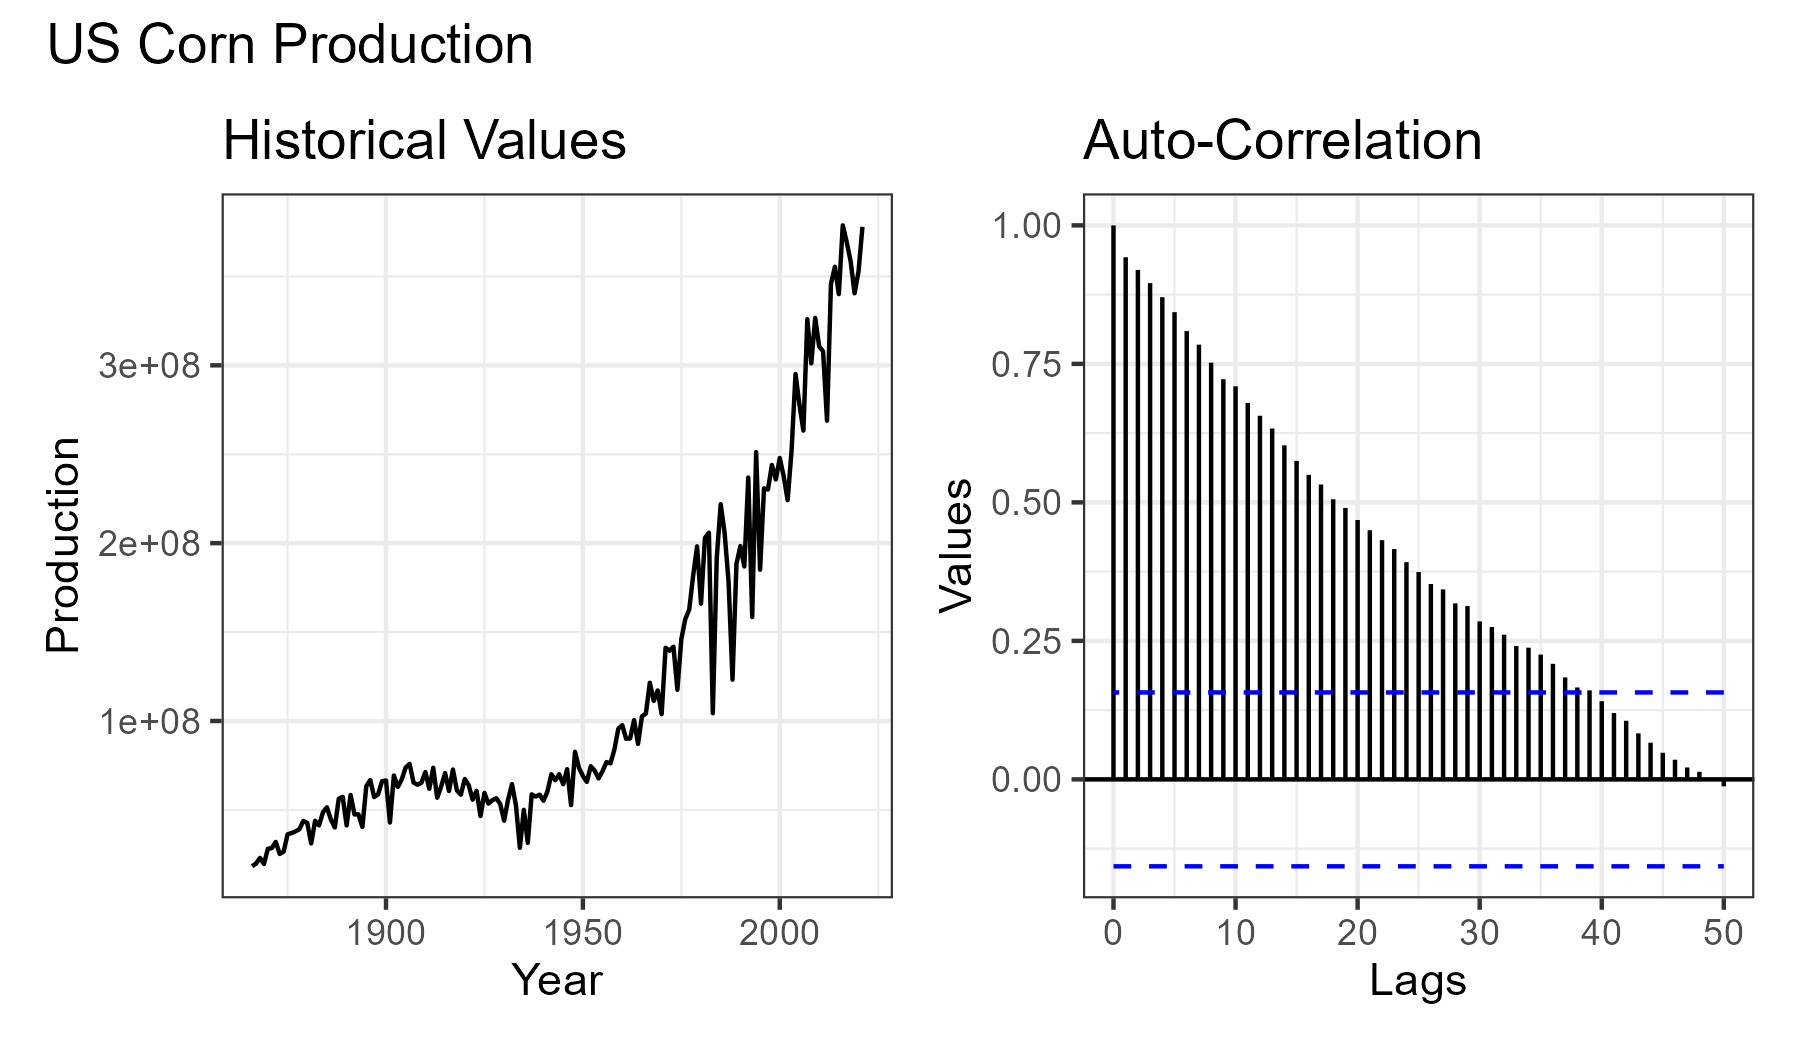
\includegraphics[width=0.8\textwidth]{figures/corn_prod.png}
\end{figure}

Now for the test, we use the function \href{https://rdrr.io/cran/aTSA/man/adf.test.html}{aTSA::adf.test}, that tests three specifications:

\begin{itemize}
    \item Type 1: A linear model with no drift nor linear trend.
    \item Type 2: A linear model with drift but no linear trend.
    \item Type 3: A linear model with drift and linear trend.
\end{itemize}

Each of them with a multitude of lags of the first difference of the serie. In our case, I set the maximum number of lags to 4, given the yearly nature of the data.

Test statistic is the estimated coefficient of the lagged time serie, divided by its standard error. The null hypothesis is that the coefficient is equal to zero, which would indicate an $I(0)$ process.

The results are presented below, with p-values in parenthesis. We can see that the null hypothesis is rejected for all three specifications, for any number of lags, which indicates that the series has a unit root.


% Table created by stargazer v.5.2.3 by Marek Hlavac, Social Policy Institute. E-mail: marek.hlavac at gmail.com
% Date and time: sáb, mai 18, 2024 - 17:42:28
\begin{table}[!htbp] \centering 
  \caption{} 
  \label{} 
\begin{tabular}{@{\extracolsep{5pt}} cccc} 
\\[-1.8ex]\hline 
\hline \\[-1.8ex] 
Lag & Type 1 & Type 2 & Type 3 \\ 
\hline \\[-1.8ex] 
0 & 0.61
(0.82) & -0.54
(0.86) & -2.74
(0.27) \\ 
1 & 2.08
(0.99) & 0.78
(0.99) & -1.16
(0.91) \\ 
2 & 3.01
(0.99) & 1.51
(0.99) & -0.53
(0.98) \\ 
3 & 3.91
(0.99) & 2.21
(0.99) & 0
(0.99) \\ 
4 & 4.87
(0.99) & 3.05
(0.99) & 0.54
(0.99) \\ 
\hline \\[-1.8ex] 
\end{tabular} 
\end{table} 



\end{document}
